% ============================================================================
% Standalone subsection: using $C \times a_n$ to detect RLHF-induced diversity
% loss across the OLMo-2-7B four-stage pipeline.
%
% Generated numbers come from:
%   results/rlhf_experiment/paper_macros_rlhf.tex   (\olmo* macros)
%   results/rlhf_experiment/tables/rlhf_diversity.tex  (\input'd below)
%
% Figures:
%   figures/rlhf_experiment/ak_curves_overlay_*.pdf
%   figures/rlhf_experiment/per_prompt_D_violin_*.pdf
%   figures/rlhf_experiment/metric_correlation_scatter_*.pdf
%
% This file is NOT \input by paper/in_context_diversity_metric.tex yet.
% Matthew will decide when / where to add the \input.
% ============================================================================

\section{Detecting Post-Training Diversity Loss on OLMo-2-7B}\label{sec:rlhf-experiment}

Prior sections validated $D = C \times a_n$ on synthetic response sets and on Tevet and Berant's human-labelled diversity sets. Here we close the gap flagged in Section~\ref{sec:exp-discussion}: sample from real policies at different post-training stages and ask whether $D$ detects the diversity loss widely attributed to RLHF \citep{kirk2023rlhf,zhang2025verbalizedsampling,padmakumar2023writingreduces}.

\paragraph{Setup.} We sample from the four released stages of the OLMo-2-1124-7B pipeline \citep{olmo2024olmo2}: the pretrained base model, its SFT checkpoint, the DPO checkpoint trained on preference data, and the final RLVR-tuned Instruct checkpoint. On two prompt sets --- \olmoAlpacaN{} AlpacaEval prompts (seed=42 subsample of 805) \citep{dubois2024alpacaeval} and \olmoNbCuratedN{} curated NoveltyBench prompts \citep{zhang2025noveltybench} --- we draw $K{=}10$ responses per prompt per stage (temperature 1.0, top-$p$ 1.0, $\texttt{max\_new\_tokens}{=}100$). Base runs raw; SFT / DPO / Instruct receive the prompt through their own chat template. We score each (stage, prompt) group with $D = C \times a_n$ using Qwen2.5-3B as $\theta$ and 25 permutations (a 5-prompt spot check at 50 permutations confirmed per-prompt rank stability). For comparison we also compute Kirk et al.'s EAD and distinct-$n$ (averaged over $n{=}1\ldots5$) and SentBERT similarity-to-diversity \citep{reimers2019sbert}.

\paragraph{Hypotheses.} Following Dror et al.'s 2018 NLP significance-testing guide \citep{dror2018hitchhiker}, we pre-register three one-sided paired Wilcoxon signed-rank tests with Bonferroni correction ($\alpha = 0.05/3$):

\begin{itemize}[nosep]
    \item \textbf{H1a} $D_{\mathrm{base}} > D_{\mathrm{SFT}}$ --- SFT narrows toward the helpful-assistant style.
    \item \textbf{H1b} $D_{\mathrm{SFT}} > D_{\mathrm{DPO}}$ --- DPO is trained on preference data and inherits its typicality bias \citep{zhang2025verbalizedsampling}.
    \item \textbf{H1c} $D_{\mathrm{base}} > D_{\mathrm{RLVR}}$ --- cumulative effect of the full post-training pipeline.
\end{itemize}

The DPO-vs-RLVR comparison is reported as an exploratory two-sided contrast (H1$'$): RLVR uses \emph{verifiable} rewards (math / code / instruction-following) rather than human preferences, so the typicality-bias argument that motivates H1b does not obviously apply to it, and the effect direction is genuinely open.

\paragraph{Results.}

\begin{table}[h]
\centering
\caption{Per-prompt $D = C \times a_n$ by OLMo-2-7B stage, with pre-registered paired tests.}
\label{tab:rlhf-diversity}
\small
\begin{tabular}{lrrr}
\toprule
Stage & $D = C \cdot a_n$ mean & std & $n$ \\
\midrule
Base & 0.488 & 0.045 & 200 \\
SFT & 0.330 & 0.093 & 200 \\
DPO & 0.290 & 0.068 & 200 \\
Instruct (RLVR) & 0.285 & 0.071 & 200 \\
\midrule
\multicolumn{4}{l}{\textbf{H1 tests (paired Wilcoxon, Bonferroni)}} \\
Base$>$ SFT & $\Delta=0.158$ & $d_z=1.614$ & $p=<0.001$ \\
SFT$>$ DPO & $\Delta=0.040$ & $d_z=0.577$ & $p=<0.001$ \\
Base$>$ Instruct (RLVR) & $\Delta=0.202$ & $d_z=2.526$ & $p=<0.001$ \\
\multicolumn{4}{l}{\textbf{H1' (exploratory two-sided, uncorrected)}} \\
DPO $\neq$ Instruct & $\Delta=0.005$ & $d_z=0.222$ & $p=<0.001$ \\
\bottomrule
\end{tabular}

\vspace{0.5em}

\begin{tabular}{lrrr}
\toprule
Stage & $D = C \cdot a_n$ mean & std & $n$ \\
\midrule
Base & 0.498 & 0.030 & 100 \\
SFT & 0.384 & 0.089 & 100 \\
DPO & 0.318 & 0.073 & 100 \\
Instruct (RLVR) & 0.315 & 0.086 & 100 \\
\midrule
\multicolumn{4}{l}{\textbf{H1 tests (paired Wilcoxon, Bonferroni)}} \\
Base$>$ SFT & $\Delta=0.113$ & $d_z=1.232$ & $p=<0.001$ \\
SFT$>$ DPO & $\Delta=0.066$ & $d_z=0.897$ & $p=<0.001$ \\
Base$>$ Instruct (RLVR) & $\Delta=0.183$ & $d_z=2.054$ & $p=<0.001$ \\
\multicolumn{4}{l}{\textbf{H1' (exploratory two-sided, uncorrected)}} \\
DPO $\neq$ Instruct & $\Delta=0.004$ & $d_z=0.069$ & $p=0.016$ \\
\bottomrule
\end{tabular}

\vspace{0.5em}

\end{table}

Table~\ref{tab:rlhf-diversity} reports per-stage means, the pre-registered contrasts, and the exploratory DPO$\,\neq\,$RLVR test. On AlpacaEval, $D$ drops from \olmoAlpacaBaseDMean{} (base) to \olmoAlpacaSftDMean{} (SFT) to \olmoAlpacaDpoDMean{} (DPO) to \olmoAlpacaInstructDMean{} (Instruct/RLVR); the full-pipeline drop base$\,\rightarrow\,$RLVR has effect size $d_z = \olmoAlpacaHoneCDz$ and $p_\mathrm{Bonf} = \olmoAlpacaHoneCPbonf$. On NoveltyBench curated the corresponding means are \olmoNbCuratedBaseDMean / \olmoNbCuratedSftDMean / \olmoNbCuratedDpoDMean / \olmoNbCuratedInstructDMean with $d_z = \olmoNbCuratedHoneCDz$ and $p_\mathrm{Bonf} = \olmoNbCuratedHoneCPbonf$.

\begin{figure}[h]
\centering
\begin{subfigure}[t]{0.48\textwidth}
    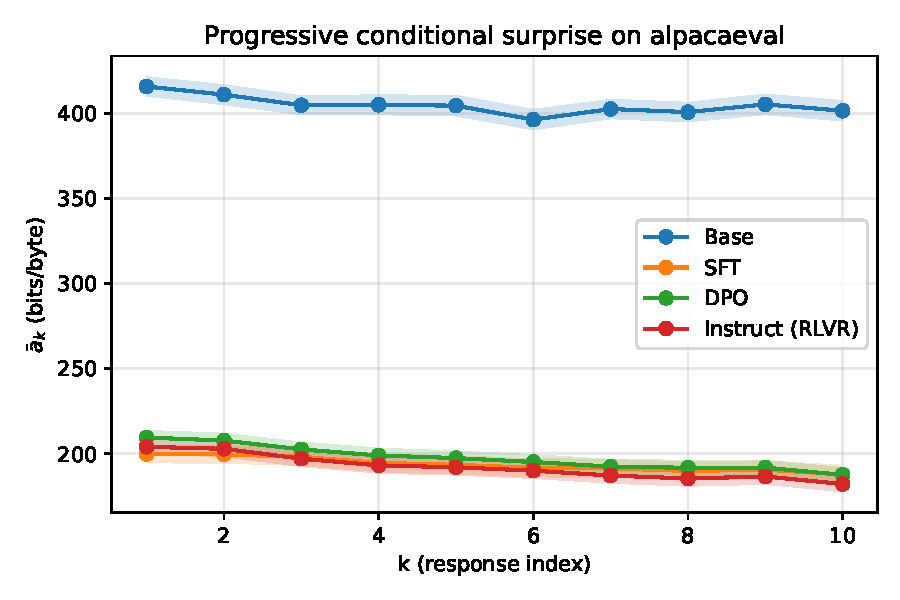
\includegraphics[width=\textwidth]{../figures/rlhf_experiment/ak_curves_overlay_alpacaeval.pdf}
    \caption{AlpacaEval $\bar{a}_k$ curves.}
\end{subfigure}\hfill
\begin{subfigure}[t]{0.48\textwidth}
    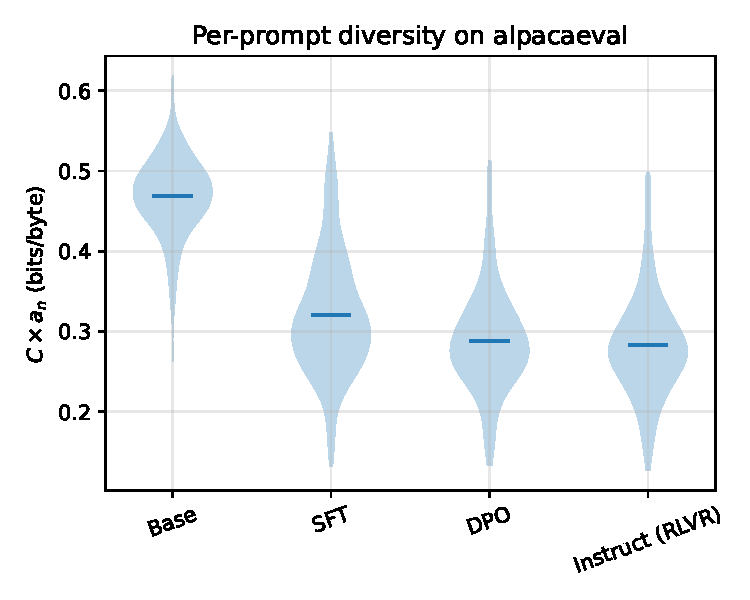
\includegraphics[width=\textwidth]{../figures/rlhf_experiment/per_prompt_D_violin_alpacaeval.pdf}
    \caption{Per-prompt $D$ by stage.}
\end{subfigure}
\caption{Progressive conditional surprise curves and per-prompt diversity distributions across the four OLMo-2-7B stages on AlpacaEval. Each later stage's $\bar{a}_k$ curve lies below the base curve at every $k \geq 2$; the per-prompt $D$ distribution shifts toward lower values as the pipeline advances.}
\label{fig:rlhf-ak-violin}
\end{figure}

\begin{figure}[h]
\centering
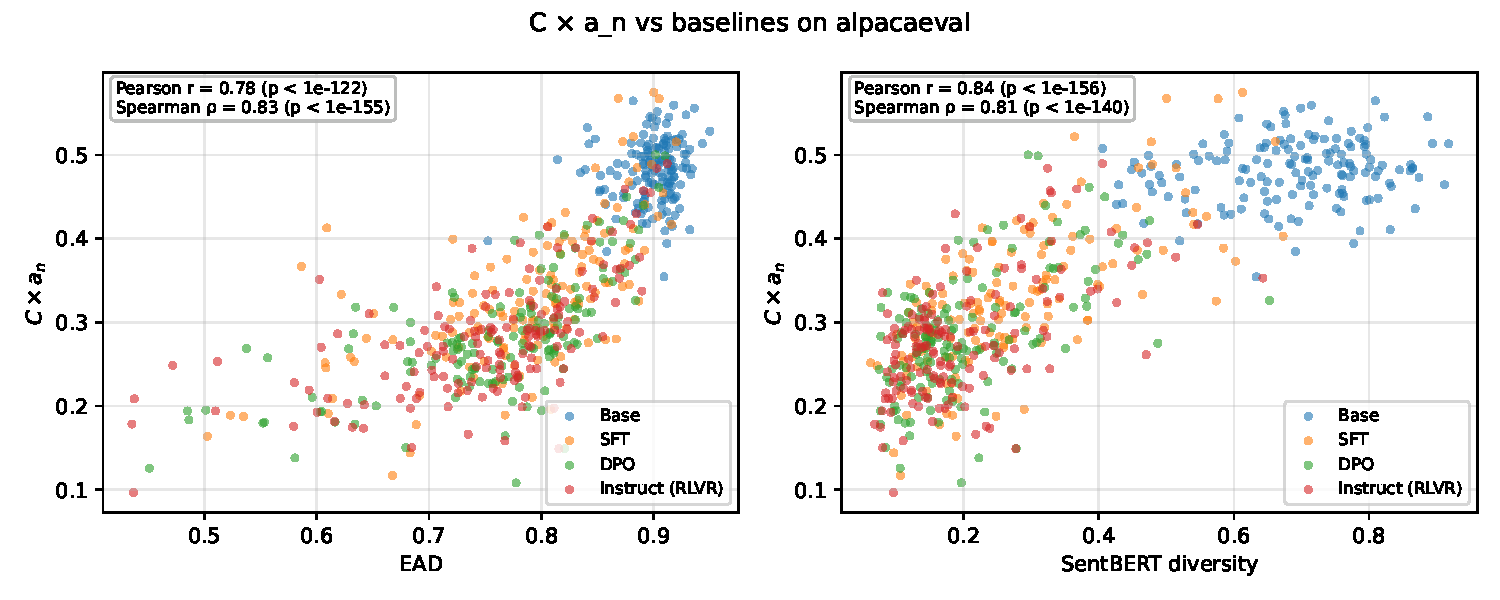
\includegraphics[width=0.8\textwidth]{../figures/rlhf_experiment/metric_correlation_scatter_alpacaeval.pdf}
\caption{Per-prompt $D = C \times a_n$ versus EAD (left) and SentBERT-similarity diversity (right) on AlpacaEval, coloured by stage. The signs and stage-ordering agree across metrics; $D$ tracks the same diversity-loss direction that EAD and SentBERT detect.}
\label{fig:rlhf-metric-scatter}
\end{figure}

\paragraph{Discussion.} The monotone drop across all three pre-registered contrasts is consistent with the post-training-reduces-diversity findings of \citet{kirk2023rlhf,padmakumar2023writingreduces}, now measured by an information-theoretic metric that needs neither an embedding model nor a sentence similarity function. Cross-metric agreement with EAD and SentBERT (H2, Figure~\ref{fig:rlhf-metric-scatter}) confirms $C \times a_n$ responds to the same signal lexical and semantic baselines detect. The DPO vs RLVR exploratory contrast is reported without pre-registered direction because RLVR's verifiable-rewards objective breaks the typicality-bias mechanism that narrows preference-trained policies; we observe $\Delta = \olmoAlpacaHpaDiff$ with $d_z = \olmoAlpacaHpaDz$.

\paragraph{Released artifacts.} The \olmoAlpacaN$\,+\,$\olmoNbCuratedN{} prompts $\times$ 4 stages $\times$ $K{=}10$ generations are released as a public HuggingFace dataset (schema compatible with NoveltyBench submissions). To our knowledge this is the first public release of $K\!\ge\!10$ sampled responses across a paired SFT/DPO/RL pipeline, filling a gap that blocked direct diversity replication of \citet{kirk2023rlhf} (whose K=16 generations were logged only to a private W\&B project).

% --- provide macro fallbacks so \input'ing this file without the generated
%     macros still compiles (the '??' placeholders signal "run the analysis") ---
\providecommand{\olmoAlpacaN}{200}
\providecommand{\olmoNbCuratedN}{100}
\providecommand{\olmoAlpacaBaseDMean}{??}
\providecommand{\olmoAlpacaSftDMean}{??}
\providecommand{\olmoAlpacaDpoDMean}{??}
\providecommand{\olmoAlpacaInstructDMean}{??}
\providecommand{\olmoAlpacaHoneCDz}{??}
\providecommand{\olmoAlpacaHoneCPbonf}{??}
\providecommand{\olmoAlpacaHpaDiff}{??}
\providecommand{\olmoAlpacaHpaDz}{??}
\providecommand{\olmoNbCuratedBaseDMean}{??}
\providecommand{\olmoNbCuratedSftDMean}{??}
\providecommand{\olmoNbCuratedDpoDMean}{??}
\providecommand{\olmoNbCuratedInstructDMean}{??}
\providecommand{\olmoNbCuratedHoneCDz}{??}
\providecommand{\olmoNbCuratedHoneCPbonf}{??}
